\documentclass[tikz]{standalone}
%\usepackage{tikz}

% tikz setup
\usetikzlibrary{automata, positioning, arrows}

\tikzset{%
    ->,
    >=stealth',
    node distance=2cm,
    .every state/.style={thick, fill=gray!10},
    initial text=$ $,
}

\begin{document}
    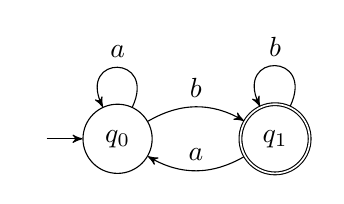
\begin{tikzpicture}
        \node[state, initial] (q0) {$q_0$};
        \node[state, accepting, right of=q0] (q1) {$q_1$};

        \draw (q0) edge[above, in=115, out=65, looseness=5] node {$a$} (q0)
        (q0) edge[above, bend left] node {$b$} (q1)
        (q1) edge[above, in=115, out=65, looseness=5] node {$b$} (q1)
        (q1) edge[above, bend left] node {$a$} (q0)
        ;
    \end{tikzpicture}
\end{document}